\section{Programmgröße}
\label{sec:eval_size}
Bei der Konstruktion eines Entscheidungsbaumes erhöht jede Teilung die Klassifizierungsgenauigkeit auf der Trainingsmenge und die Programmgröße die der Entscheidungsbaum benötigt. Folglich, sollte der verfügbare
Programmspeicher vollständig ausgenutzt werden. Die Klassifizierungsgenauigkeit muss folglich maximiert werden, unter der Bedingung, dass der Programmspeicher nicht überschritten wird. Dementsprechend müssen die Teilungen
bevorzugt werden, die den größten Zuwachs der Klassifizierungsgenauigkeit versprechen. Ein weiterer Lösungsansatz ist die Anzahl der Instruktionen pro Vergleich zu minimieren, damit mehr Vergleiche möglich sind.

\subsection{Maximierung des Zuwachses der Klassifizierungsgenauigkeit}
Scikit-Learn bietet viele Parameter an, um den Teilungsprozess bei der Konstruktion zu steuern. Einer dieser Parameter ist \texttt{min\_samples\_leaf}, d. h. die minimale Anzahl an Einträgen der Trainingsmenge
in einem Blatt. Dieser steuert die minimale Anzahl an Einträgen die in einem Kindknoten enthalten sein müssen, nachdem ein Knoten geteilt wurde. Standardmäßig ist der Wert 1. Dadurch entsteht ein sehr fein granularer
Entscheidungsbaum, der viele Blätter mit nur einem Eintrag hat. Das heißt, es wurden Teilungen durchgeführt, die nur zwei Einträge unterteilt haben. Der Zuwachs der Klassifizierungsgenauigkeit ist durch diese
Teilungen sehr gering. Eine Erhöhung in der Blattgröße verspricht, dass Entscheidungsbäume gefunden werden können, die zwar tiefer sind, aber dafür eine bessere Klassifizierungsgenauigkeit pro Vergleich erzielen.
Der Baum kann tiefer werden, da die Grenze des Programmspeichers noch nicht erreicht wurde.
\newline
\newline
Abbildung \ref{fig:msl} zeigt, wie sich der Parameter auf verschieden große Trainingsmengen auswirkt. Betrachtet wird eine Maximalhöhe von 16. Besonders bei großen Trainingsmengen (Abbildung \ref{subfig:msl_big})
kann die Programmgröße mit einer Blattgröße von 8 signifkant sinken, ohne die maximale Baumhöhe zu beeinflussen. Bei kleinen Trainingsmengen (Abbildung \ref{subfig:msl_small}) reduziert bereits bei kleinen Blattgrößen
sich die Programmgröße ebenfalls signifikant. Allerdings wird die maximale Baumhöhe beeinflusst. Besonders bei großen Trainingsmengen wirkt sich der Parameter stärker auf die Programmgröße aus.
Vermutlich, da die Anzahl der Blätter sich signifikant erhöht, je tiefer der Baum ist.
\subfigbox{
\subfigure[Trainingsmengengröße: 1023]{\label{subfig:msl_small}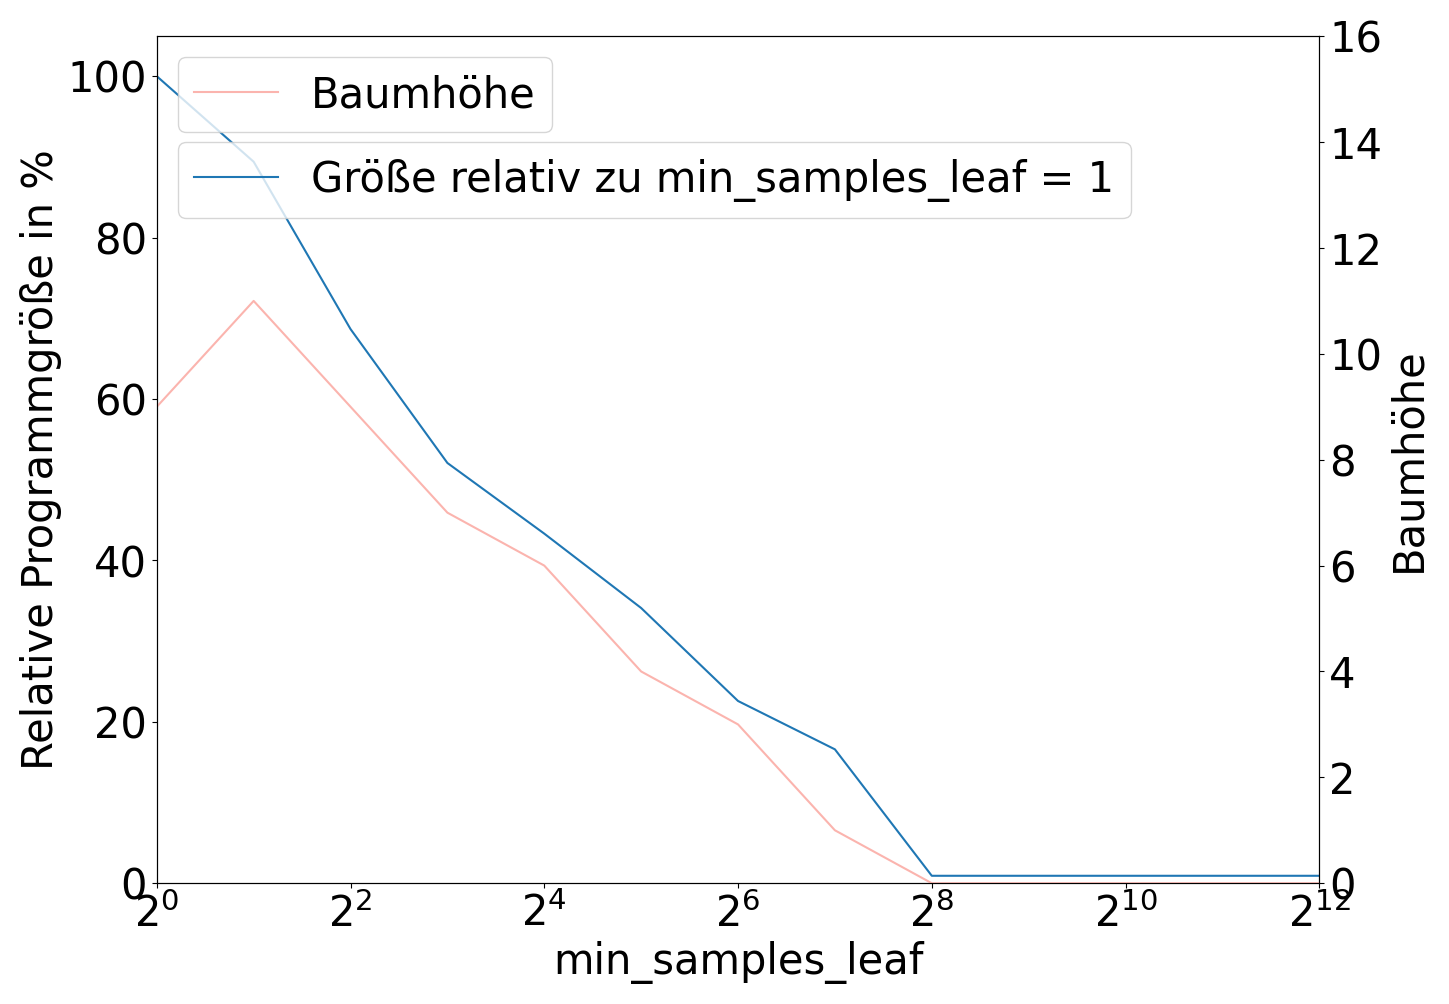
\includegraphics[width=0.48\linewidth]{images/min_samples_leaf_small.png}}\hfill%
\subfigure[Trainingsmengengröße: 7629]{\label{subfig:msl_big}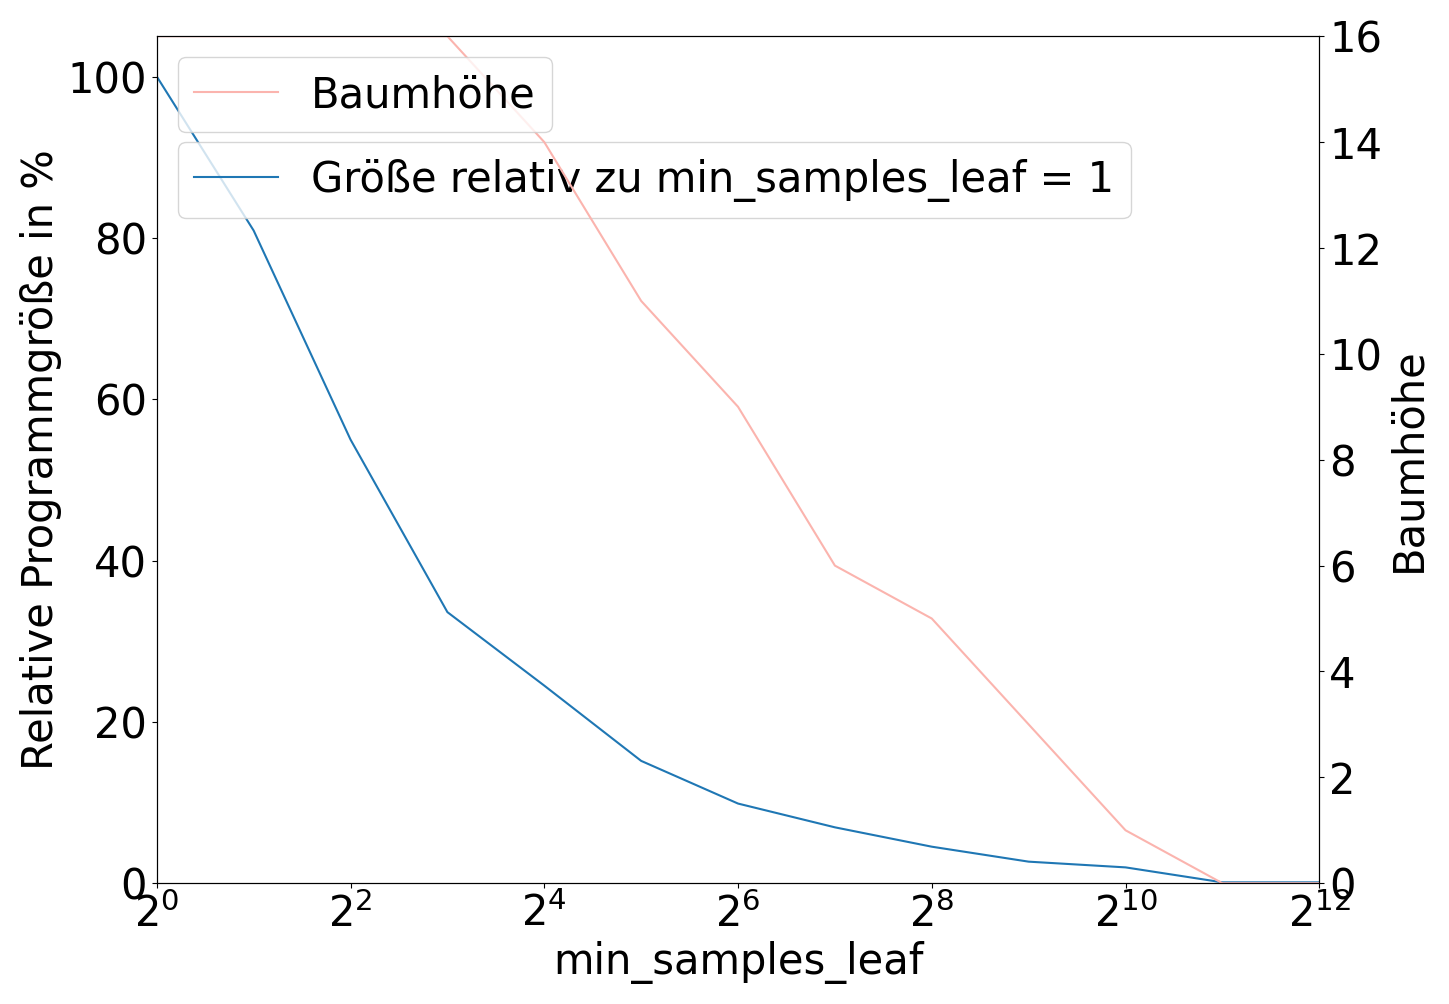
\includegraphics[width=0.48\linewidth]{images/min_samples_leaf_big.png}}%
}{Auswirkung der minimalen Blattgröße auf Programmgröße und Baumhöhe.}{fig:msl}
\newline
\newline
Es kann nicht argumentiert werden, dass ein Wert für die Blattgröße besser ist als ein Anderer, da die Klassifizierungsgenauigkeit auf der Trainingsmenge keine Aussage über die Klassifizierungsgenauigkeit auf
der Testmenge treffen kann. Eine hohe Klassifizierungsgenauigkeit auf Trainingsmenge muss nicht umbedingt eine hohe Klassifizierungsgenauigkeit auf der Testmenge implizieren. Allerdings können so vermeintlich
höhere Entscheidungsbäume ausgewählt werden, da diese weniger Programmspeicher benötigen im Vergleich zu gleich hohen Entscheidungsbäumen mit einer geringeren Blattgröße. Dieser Parameter vergrößert folglich
den Suchraum. Bei kleinen Trainingsmengen ist eine Blattgröße über 1 nur sinnvoll, wenn der größte Entscheidungsbaum, der generiert werden kann, nicht innerhalb der Restriktionen des Programmspeichers liegt.
\subsection{Minimierung der Instruktionen eines Vergleichs}
Ein Vergleich in einem Entscheidungsbaum wurde in Kapitel \ref{sec:cCodeTree} als Abzweigungsexpression mit einem Test definiert. Der Compiler erzeugt für den gleichen Programmcode verschieden viele Instruktionen
je nach Wahl des Datentyps.
\newline
\newline
Listing \ref{lst:assemblyVergleich} zeigt die Komplexität eines einzigen Vergleichs in Instruktionen eines Gleitkommazahlvergleichs. Zeile 1 bis 4 lädt die konstante Gleitkommazahl in 4 hintereinander liegende
8-Bit Register. Zeile 5 bis 7 lädt den Zeiger, der auf die Feature-Menge zeigt, und inkrementiert ihn um 36, um auf das 9. Feature zuzugreifen. In Zeile 8 bis 11 wird das Feature in die Register geladen. Zeile 12 bis 15 führen die
Vergleichsfunktion aus. Damit benötigt ein Vergleich insgesamt 15 Instruktionen.
\begin{lstlisting}[label=lst:assemblyVergleich,caption={Vergleich von Feature als Gleitkommazahl mit konstanter Gleitkommazahl.}]
01: ldi r18,lo8(33)
02: ldi r19,lo8(-92)
03: ldi r20,lo8(69)
04: ldi r21,lo8(60)
05: ldd r26,Y+5
06: ldd r27,Y+6
07: adiw r26,36
08: ld r22,X+
09: ld r23,X+
10: ld r24,X+
11: ld r25,X
12: sbiw r26,36+3
13: call __lesf2
14: cp __zero_reg__,r24
15: brge .+2
\end{lstlisting}
Zu vermeiden sind Zeile 5 bis 11, indem alle Features nur einmal in Register geladen werden. Dies ist allerdings nur möglich, wenn die Größe der Feature-Menge nicht 32~Byte übersteigt bei dem
ATmega328P. Zusätzlich müssten noch Bytes verfügbar sein, um die Konstanten zu laden. Die Feature-Menge der Schwerpunktverteilung beinhaltet 10 Einträge. Der Ansatz mit Gleitkommazahlen ist mit 40 Bytes zu groß.
Der Ansatz mit Ganzzahlen kann diese Optimierung mit 20~Byte ausnutzen. Der Compiler führt diese Optimierung bereits automatisch durch. Wenn die Feature-Menge zu groß ist, werden aus diesem Grund regelmäßig
Register verdrängt, wodurch zusätzlich Instruktionen entstehen. Die Anzahl der Instruktionen können reduziert werden, indem die Größe der Feature-Menge reduziert wird, sodass die Feature-Menge und eine
zusätzliche Konstante des gleichen Datentyps den Registerspeicher nicht übersteigen.
\newline
\newline
Der Datentyp \texttt{Float} ist sehr teuer für einen 8-Bit Prozessor, da immer 4~Register benötigt werden und gegebenenfalls zusätzliche Funktionen, die die fehlende Hardwareunterstüzung ergänzen.
Idealerweise sollte für die Feature-Menge und die Vergleiche ein 8-Bit Datentyp gewählt werden. Damit werden einerseits weniger Register benötigt, wodurch wiederrum die Feature-Menge größer sein kann,
und andererseits können hardwareunterstützte Vergleichsinstruktionen benutzt werden. Dies verringert die Anzahl der Instruktionen signifikant. Folglich vermindert ein kleinerer Datentyp die Anzahl der
Instruktionen signifikant. Listing \ref{lst:assemblyVergleich8Bit} zeigt einen Vergleich von einem 8-Bit Datentyp. Im Kontrast zum Vergleich mit Gleitkommazahlen, werden 66,6\% weniger Instruktionen
benötigt.
\begin{lstlisting}[label=lst:assemblyVergleich8Bit,caption={Vergleich von 8-Bit Feature mit konstanter 8-Bit Zahl.}]
01: adiw r26,4
02: ld r24,X
03: sbiw r26,4
04: cpi r24,lo8(124)
05: brge .L3
\end{lstlisting}
\subsection{Minimierung der Instruktionen einer Rückgabe}
Die Rückgabe der Klassifizierung in einem Entscheidungsbaum kann auf zwei Arten stattfinden. Einerseits kann lediglich die Klasse mit der höchsten Wahrscheinlichkeit zurückgegeben werden. Andererseits kann die
Wahrscheinlichkeitsverteilung zurückgegeben werden, sodass die nächste Ebene die Entscheidung trifft. In Kapitel \ref{sec:cCodeTree} wurde letzteres vorgestellt, da in der nächsten Ebene der Wahlklassifizierer
die Entscheidungsbäume im Ensemble mit Hilfe ihrer Wahrscheinlichkeitsverteilungen zusammenfasst.
\newline
\newline
Listing \ref{lst:assemblyBlattReturn} zeigt die Instruktionen die für die Zuweisung zu vier Klassen von 1.0, 0.0, 0.0 und 0.0 generiert werden. Für jede Klasse wird die Konstante Wahrscheinlichkeit in Register geladen
und anschließend in den Rückgabeparameter gespeichert. In diesem Fall muss nur für die erste Klasse eine Konstante geladen werden, da jede andere Klasse 0 ist. Das heißt, dass im schlimmsten Fall 33
Instruktionen benötigt werden, anstatt 21. Der Compiler führt hier bereits eine Optimierung aus, indem für jedes Ergebnis ein eigener \textit{Basic block} (Eine Datenstruktur die Instruktionen mit einer Annotation
zusammenfasst)erzeugt wird. Zusätzlich könnte kein C-Code generiert werden für eine Zuweisungen mit 0. Dies erfordert aber, dass der Rückgabeparameter mit 0 vorinitialisiert ist.
\newpage
\begin{lstlisting}[label=lst:assemblyBlattReturn,caption={Beispiel der Instruktionen einer Rückgabe der Wahrscheinlichkeitsverteilung eines Entscheidungsbaumes mit 4~Klassen.}]
01: ldi r24,0
02: ldi r25,0
03: ldi r26,lo8(-128)
04: ldi r27,lo8(63)
05: st Z,r24
06: std Z+1,r25
07: std Z+2,r26
08: std Z+3,r27
09: std Z+4,__zero_reg__
10: std Z+5,__zero_reg__
11: std Z+6,__zero_reg__
12: std Z+7,__zero_reg__
13: std Z+8,__zero_reg__
14: std Z+9,__zero_reg__
15: std Z+10,__zero_reg__
16: std Z+11,__zero_reg__
17: std Z+12,__zero_reg__
18: std Z+13,__zero_reg__
19: std Z+14,__zero_reg__
20: std Z+15,__zero_reg__
21: ret
\end{lstlisting}
Eine weitere Optimierung ist den Wahlklassifizierer diskret zu modellieren. Dabei wird für jede Rückgabe des Entscheidungsbaumes ein einstimmiges Ergebnis angenommen, d. h. es wird die Klasse mit der
höchsten Wahrscheinlichkeit in jedem Baum zurückgegeben und nicht mehr die Wahrscheinlichkeitsverteilung. Dadurch werden lediglich die erkannten Klassen
gezählt, anstatt die Wahrscheinlichkeitsverteilungen zu addieren. Listing \ref{lst:assemblyBlattReturnDiskret} zeigt, dass sich die Anzahl der Instruktionen für eine Rückgabe auf genau 2~Instruktionen
reduzieren. Zusätzlich kann der Compiler diese Rückgabe in Basic blocks extrahieren, wodurch lediglich eine Sprunginstruktion benötigt wird. Diese Optimierung ist bei dem diskreten Wahlklassifizierer noch
effektiver, da es genau $N$ verschiedene Rückgabewerte gibt, für $N$ mögliche Klassen. Im schlimmsten Fall reduzieren sich die Anzahl der Instruktionen pro Rückgabe um $\frac{100}{1 + 4N}$\%
und im besten Fall um $\frac{100}{1 + 8N}$\%.
\begin{lstlisting}[label=lst:assemblyBlattReturnDiskret,caption={Beispiel des Assemblycodes der Rückgabe eines diskreten Wahlklassifizierers.}]
01: ldi r24,lo8(1)
02: ret
\end{lstlisting}
Der Nachteil dieses Ansatzes ist, dass die Ergebnisse instabil werden können, wenn viele Rückgaben nur über eine knappe Mehrheit verfügen. Das ist insbesondere der Fall in Kombination mit einem hohen Wert
für die Blattgröße, da dieser die Anzahl der Blattknoten mit Einträgen aus verschiedenen Klassen potenziell erhöht. Diese Optimierung kann auf eine gefundene Lösung angewendet werden, die zu groß für den
Programmspeicher ist. Anschließend sollte die Klassifizierungsgenauigkeit revalidiert werden. Tests haben ergeben, dass die Klassifizierungsgenauigkeit geringfügig schwankt. Folglich kann sich die
Klassifizierungsgenauigkeit auf der Testmenge auch erhöhen.
\newline
\newline
Denkbar wäre ein hybrider Ansatz, der bei einem eindeutigen Ergebnis die Klasse zurück gibt und ansonsten die Wahrscheinlichkeitsverteilung. Die \glqq Eindeutigkeit\grqq\ kann über
einen Schwellenwert $\delta$ definiert sein. Ein Schwellenwert von $\delta=0$ würde an der Korrektheit nichts ändern, würde aber im schlimmsten Fall die Programmgröße nicht verringern.
Tests haben ergeben, dass es immer eindeutige Ergebnisse gibt, weswegen diese Optimierung immer angewendet werden sollte.
